\documentclass[12pt,a4paper,onecolumn,titlepage,twoside,openany]{book}
% \usepackage[utf8]{vietnam}
%\usepackage{fouriernc}
\usepackage{tasks}
%%%%%%%%%%%% KIỂU MÀU VÀ ĐỘ RỘNG NOTE
% \def\kieumau{Y} %Y: Màu; N: đen-trắng
% \def\kieumau{N} %Y: Màu; N: đen-trắng
\def\kieumau{P}
\usepackage{xcolor} 
\def\leftnote{5} %Độ rộng cột Note
%%%%%%%%%%%%% ĐN CƠ BẢN
\input{cautrucDT/color\kieumau} %MÀU
\input{cautrucDT/Khai-bao-cho-file-mainDT} %Khai báo cơ bản
\usepackage{currfile}
\usepackage{tkz-euclide,circuitikz}
\usepackage{chessfss}
\usepackage{wrapfig}
%%%%%%%%%%%%% ĐIỀU KHIỂN LỜI GIẢI ,DÒNG CHẤM, ĐÁP SỐ
%------------Dòng chấm bằng chiều dài LG (bật)
% \dotlinefull{ex}
% \dotlinefull{vd}
%------------Thay Loi giải bằng n dòng kẻ (bật)
% \dotlineans{5}{ex}
%------------Ẩn lời giải
% \hideansEX{vd}
%------------Dòng chấm tùy ý (ko cần \loigiai{})
%---Nhiều câu cùng dòng chấm (tách dụng lên mọi đề)
% \dongchamEXS{1,...,216}{3}
% \dongchamEXS{217,...,288}{2}
%---Nhiều câu cùng dòng chấm (tách dụng lên MỘT ĐỀ đc chọn)
%\DEdongchamEXS{3}{1,...,20}{2} %{3} là đề thứ 3
%---Dòng chấm từng câu, tác dụng lên mọi đề
%\dongchamEX{1/3,2/5,3/7} % câu / số dòng chấm của câu đó
%---Dòng chấm từng câu, tác dụng lên 1 đê
%\DEdongchamEX{3}{1/3,2/5,3/7} % câu / số dòng chấm của câu đó, {3} là đề số 3 

% \showansEX{vd}[1,3,7,8,9,13,17,20,24,26,29,43,46,50,51,52,53,54,63,64]
%------------Ẩn đáp số (bật), đáp án
\exitdapso %ẩn đs
%\renewcommand{\indapan}[2]{} %ẩn đáp án
%%%%%%%%%%%%% khung NAME
\def\hoten{Gọi tôi là:}
\def\ngaylamde{Ngày làm đề: ...../...../........} %để {} nếu ko muốn
\def\tenchude{GIẢI ĐỀ TUYỂN SINH VÀO LỚP 10 GIA LAI}
\def\tendethi{ÔN TẬP TS 10}
\def\tentruong{LỚP TOÁN THẦY PHÁT}
\def\thoigian{Thời gian làm bài: 120 phút}
%%%%%%%%%%%%% Nội dung head & foot
% \def\diachi{ }
\def\diachi{VNPmath - 0962940819}
\def\tenchuyende{\tenchude}
\def\tentacgia{GV.VŨ NGỌC PHÁT}
\def\chamngon{\lq\lq  It's not how much time you have, it's how you use it.\rq\rq
}
% \def\QRde{12THQG-ST}
% 
\includegraphics{QRcode/12THQG-ST.png}
%%%%%%%%%%%%% Đn lại A.B.C.D
\khoanhtrondapan
% \khongkhoanhtrondapan
%%%%%%%%%%%%%
\renewcommand{\arraystretch}{1}
%TF Option
\OPTN{kindTF=t,dapanTF=a,boldTF=1,phatbieu=Mệnh đề,viettat=1}
% \OPTN{kindSA=oly,ketquaSA=KQ:,widthSA=4,heightSA=0.9,dapanSA=a}
% 
%%===================================================
% \usepackage{tabularray}
%=================BẮT ĐẦU TÀI LIỆU===================
\makeatletter
\everymath{\color{mauD}}

\begin{document}
\renewcommand{\chaptername}{Chương}
\pagenumbering{arabic}%đánh số trang dạng 1,2,...
%====================================================
%==================BẮT ĐẦU TÀI LIỆU==================
%\hienEXS{41}{50} %chỉ hiện câu từ 41 đến 50 của đề
%--------Đề bài
% \setcounter{deso}{5}
% \NOTE \anLG \anDA
% \tableofcontents
\FULLWIDTH \anLG \anDA

% --
% \notename


\begin{vd}
	

    Cho biết công $A$ (đơn vị: $J$) sinh bởi lực $\vec{F}$ tác dụng lên một vật được tính bằng công thức $A = \vec{F}\cdot\vec{d}$, trong đó $\vec{d}$ là vectơ biểu thị độ dịch chuyển của vật (đơn vị của $\left|\vec{d}\right|$ là m) khi chịu tác dụng của lực $\vec{F}$.
	
	Một chiếc xe có khối lượng $1{,}5$ tấn đang đi xuống trên một đoạn đường dốc có góc nghiêng $5^\circ$ so với phương ngang. Tính công sinh bởi trọng lực $\vec{P}$ khi xe đi hết đoạn đường dốc dài $30$ m (làm tròn kết quả đến hàng đơn vị), biết rằng trọng lực $\vec{P}$ được xác định bởi công thức $\vec{P} = m\vec{g}$, với $m$ (đơn vị: kg) là khối lượng của vật và $\vec{g}$ là gia tốc trọng trường có độ lớn $g = 9{,}8$ m/s$^2$.
	\dongcham{4}
	\loigiai{
	\begin{center}
	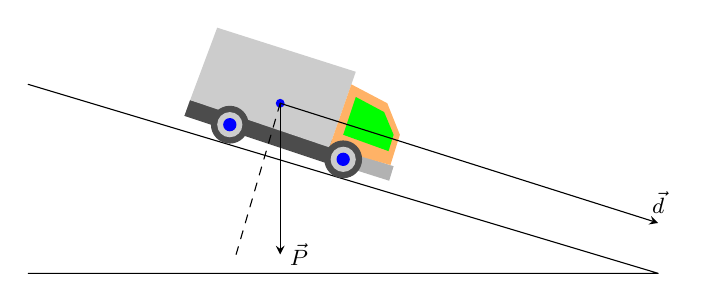
\begin{tikzpicture}[scale=0.8,font=\footnotesize, line join=round, line cap=round, >=stealth]
	\def\xe{orange!60}
	\def\den{red}
	\draw (0,3)--(10,0) (0,0)--(10,0);
	\fill[black!30] (2.48,2.5)--(2.57,2.75)--(5.8,1.7)--(5.73,1.47)--cycle ;
	\fill[black!70] (2.48,2.5)--(2.57,2.75)--(5.2,2)--(5.18,1.6)--cycle ;
	\fill[black!20] (2.57,2.75)--(3,3.9)--(5.2,3.2)--(4.78,2)--cycle ;
	\fill[\xe] (4.78,2)--(5.13,3)--(5.7,2.7)--(5.9,2.2)--(5.75,1.72)--cycle ;
	\fill[green] (5.2,2.8)--(5.65,2.56)--(5.8,2.2)--(5.72,1.94)--(5,2.2)--cycle ;
	\fill[black!70] (3.2,2.36) circle (0.3) (5,1.81) circle (0.3) ;
	\fill[black!20] (3.2,2.36) circle (0.2) (5,1.81) circle (0.2) ;
	\fill[blue](3.2,2.36) circle (3pt) (5,1.81) circle (3pt) (4,2.7) circle (2pt) ;
	\draw[dashed] (4,2.7)--(3.3,0.3) ;
	\draw[->] (4,2.7)--(4,0.3) node[right] {$\vec{P}$};
	\draw[->] (4,2.7)--(10,0.8) node[above] {$\vec{d}$};
	\end{tikzpicture}
	%\includegraphics{hinhanh/H1.png} 
	\end{center}
	\noindent
	Ta có $1{,}5$ tấn = $1~500$ kg.\\
	Độ lớn của trọng lực tác dụng lên chiếc xe là $\left|\vec{P}\right| = m \left|\vec{g}\right| = 1~500\cdot 9{,}8 = 14~700$ (N).\\
	Vectơ d biểu thị độ dịch chuyển của xe có độ dài là $\left|\vec{d}\right| = 30$ (m) và $ \left(\vec{P},\vec{d}\right)= 90^\circ - 5^\circ = 85^\circ$.\\
	Công sinh ra bởi trọng lực $\vec{P}$ khi xe đi hết đoạn đường dốc dài $30$ m là
	$$A=\vec{P}\cdot\vec{d}=\left|\vec{P}\right|\cdot\left|\vec{d}\right|\cdot\cos\left(\vec{P},\vec{d}\right) = 14~700\cdot 30\cdot \cos 85^\circ \approx 38~436~(J).$$
	}
\end{vd}
% 
% --------Lời giải chi tiết

% \FULLWIDTH \hienLG \hienDA % ẩn bảng đáp án
% \tableofcontents
% \newpage
% \renewcommand{\dotlineEX}[1]{}
% % % --
% \setcounter{deso}{5}

% \chap{LỜI GIẢI CHI TIẾT} \setcounter{dang}{0} \setcounter{section}{0}
% \input{input12.tex}
% ---------Mục lục chính
% \FULLWIDTH
% \vfill
% \tableofcontents %lệnh in mục lục chính
% \newpage
% \vfill
% \begin{center}
% 	
\includegraphics[width=5cm]{QRcode/12D1X2.png}
% \end{center}

\end{document}